\chapter{Études théoriques des systèmes à plusieurs corps}
\label{chap-theory}
\section{Le problème électronique}
Dans la physique des solides, on est amené à étudier l'équation de Schrödinger d'un système
à plusieurs corps ($N$ électrons et $M$ ions par exemple),
ce qui consiste à résoudre une équation du type
\begin{equation}
  \label{eqn-schrodinger}
  \qty(\sum_{i=1}^N \frac{\vb{p}_i^2}{2m_i}
  + \sum_{I=1}^M \frac{\vb{P}_i^2}{2M_I}
  + \sum_{i<j}\frac{e^2}{\abs{\vb{r}_i - \vb{r}_j}}
  - \sum_{i,I}\frac{Z_I e^2}{\abs{\vb{r}_i - \vb{R}_I}}
  + \sum_{I<J}\frac{Z_I Z_J e^2}{\abs{\vb{R}_i - \vb{R}_j}} )\Psi = E_{\V{tot}}\Psi,
\end{equation}
où $(\vb{r}, \vb{p})$ et $(\vb{R}, \vb{P})$ sont respctivement la position et l'impulsion d'un éléctron et d'un ion,
$E_{\V{tot}}$ est une certaine énergie propre du système à déterminer et enfin, la fonction d'onde
$\Psi = \Psi(\vb{r}_1, \ldots, \vb{r}_N,  \vb{R}_1, \ldots \vb{R}_M)$ est une fonction à $N+M$ variables.

Comme le système étudié (un état solide par exemple)
peut comprendre un nombre très élevé d'électrons et d'ions,
l'\cref{eqn-schrodinger} ne peut pas être résolue analytiquement, voire numériquement.
Certaines approximations doivent être appliquées au système afin de réduire la complexité du calcul.
La première approximation que l'on peut prendre, celle la plus intuitive,
est celle de Born-Oppenheimer~\cite{Born1927}.
En tenant compte du rapport de masse entre les électrons et les ions
et en supposant que les ions sont quasiment figés dans leur positions par rapport aux électrons
(ayant une longueur d'onde de De Broglie plus élevée),
on peut réécrire l'hamiltonien du système d'électrons comme
\begin{equation*}
  H = \underbrace{\sum_{i=1}^N\frac{\vb{p}_i^2}{2m_i}}_{T}
    + \underbrace{\sum_{i<j}\frac{e^2}{\abs{\vb{r}_i - \vb{r}_j}}}_{V}
    - \sum_i V_{\V{ext}}(\vb{r}_i),
\end{equation*}
où $T$ est l'énergie cinétique des électrons, $V$ leur énergie potentielle d'interaction
et $V_{\V{ext}}$ l'énergie potentielle dûe aux ions figés.
Notre problème devient donc
\begin{equation*}
  H\Psi_e(\vb{r}_1, \ldots \vb{r}_N) = E_{\V{tot}} \Psi_e(\vb{r}_1, \ldots \vb{r}_N)
\end{equation*}
Or, le problème n'est toujours pas simple car la fonction d'onde $\Psi_e$
que l'on cherche est une fonction à plusieurs variables.

\section{Théorie de la fonctionnelle de la densité}
\subsection{La méthode de Kohn et Sham}
\label{subsec-KS}
Si les électrons étaient non-interagissant entre eux,
on pourrait écrire l'hamiltonien comme une somme de plusieurs hamiltoniens d'un seul électron, \ie{}
\begin{equation}\label{eqn-H-1e}
  H = \sum_i H_i^{(1e)} = \sum_i (-\frac{\hslash^2}{2m}\laplacian_i + V_{\V{eff}}(\vb{r}_i)).
\end{equation}

Les théorèmes suivants~\cite{Hohenberg1964, Kohn1965} nous donnent la possibilité d'écrire
la vraie solution en passant par un système auxiliaire d'électrons non-interagissants.

\begin{theoreme}[Hohnenberg-Kohn~\cite{Hohenberg1964}]
  L'espérance d'un observable dans l'état fondamental est une fonctionnelle unique
  de la densité d'électrons.
\end{theoreme}

La preuve de ce théorème peut être trouvée dans~\cite{Martin2004, Sottile2003}.
Ce résultat implique que l'espérance de l'hamiltonien à l'état fondamental,
et donc l'énergie totale du système, est une fonctionnelle de la densité d'électrons
\begin{equation*}
n(\vb{r}) = \sum_i \int \abs{\Psi_e(\vb{r}_1, \ldots \vb{r}_N)}^2 \delta(\vb{r} - \vb{r}_i) \prod_{j=1}^N \dd{\vb{r}_j}.
\end{equation*}

Grâce à ce théorème, la résolution d'un système à plusieurs corps devient
la recherche d'une fonctionnelle réelle dépendant uniquement d'une variable spatiale.
La résolution va être plus simple à implémenter par rapport à la recherche de la fonction d'onde
à plusieurs variable $\Psi (\vb{r}_1, \ldots, \vb{r}_N)$ du problème initial.

\begin{theoreme}[Kohn-Sham~\cite{Kohn1965}]
\label{thm-ks}
  Pour tout système qui contient des termes d'interactions entre électrons,
  il existe un système auxiliaire non-interagissant ayant la même densité d'électrons.
\end{theoreme}

Ce théorème fournit un autre pillier de la DFT\@.
Pour un système de hamiltonian $H = T + V + V_{\V{ext}}$,
la méthode de Kohn et Sham proprose un système auxiliaire de hamiltonien $H' = T' + V'_{\V{tot}}$,
avec la même densité d'électrons que le vrai système.
Ce système auxiliaire étant non-interagissant, sa densité peut s'exprimer sous la forme
$n(\vb{r}) = n'(\vb{r}) = \sum_i \abs{\phi_i(\vb{r})}^2$

On peut donc considérer le système d'équations suivant
\begin{equation}
  \label{eqn-kseqns}
  (-\frac{1}{2}\laplacian_i + V_{\V{tot}}[n](\vb{r}))\phi_i(\vb{r}) = \epsilon_i\phi_i(\vb{r})
\end{equation}
avec
\begin{equation}
  \label{eqn-Vtot}
  V_{\V{tot}}(\vb{r}) = \underbrace{V_{\V{ext}}(\vb{r})}_\text{potentiel créé par les ions}
  + \underbrace{\int \dd{\vb{r}'} \frac{n(\vb{r}')}{\abs{\vb{r} - \vb{r}'}}}_\text{potentiel de Hatree}
  + \underbrace{V_{\V{xc}}([n], \vb{r})}_\text{potentiel d'échange-corrélation}
\end{equation}
pour chacun des électrons $i$.
Le problème devient un problème simple de $N$ équations à une variable (en $\phi_i(\vb{r})$) séparées.
On pourra ensuite faire une résolution auto-consistente en réinjectant
$n = \sum_i \abs{\phi_i^{(p)}(\vb{r})}^2 $ dans l'hamiltonien avec $\phi_i^{(p)}$
la fonction d'onde obtenue à la fin de la p-ième itération.
(Remarquons que le critère de convergence de cette méthode n'a toujours pas été trouvé.)
Cependant, il y a une approximation à faire pour le terme de potentiel d'échange-corrélation qui est dû au passage au système auxiliaire dans le \cref{thm-ks}.
Les approximations les plus couramment utilisées pour $E_{\V{xc}}$, et ainsi que pour $V_{\V{xc}}$,
sont celle des gradients généralisées (Generalized Gradient Approximations, GGA)~\cite{Langreth1980, Perdew1986, Perdew1992}
et celle de la densité locale (\textit{Local Density Approximation}, LDA)~\cite{Kohn1965},
dont nous explicitons dans la \cref{subsec-xc}.

Une fois l'énergie totale du système auxiliaire $E[n]$ minimisée,
le \cref{thm-ks} nous permettra d'obtenir la densité exacte $n(\vb{r})$ du vrai système,
ce qui détermine ensuite l'énergie de l'état fondamental.

La DFT, qui implémente numériquement les théories ci-dessus,
est aujourd'hui la méthode la plus couramment utilisée pour étudier
les propriétés de l'état fondamental d'un système
(module d'élasticité, stabilité de la structure, vibrations phononiques, etc.)~\cite{Martin2004}.

\section[TDDFT]{Théorie de la fonctionelle de la densité dépendante du temps}
\label{sec-TDDFT}
Dans les études de spectroscopie,
nous étudions les comportements des matériaux sous des perturbations externes.
Par exemple, 
la fonction diélectrique et son inverse,
qui sont déduits de l'absorption et de la réflexion des lumières~\cite{Sottile2003}
sont des grandeurs physiques auxquelles l'on s'intéresse beaucoup dans les expériences.
Par conséquent, une simple étude de l'état fondamental ne suffit pas,
il nous faut de plus des études sur les états excités.

La méthode que nous allons présenter dans la suite,
la théorie de la fonctionelle de la densité dépendante du temps
(\textit{Time-Dependent Density Functional Theory}, TDDFT),
est utilisée dans le code à l'aide duquel nos simulations numériques \textit{ab initio} sont effectués.
La TDDFT est une extension de la DFT\@.
Grâce au théorème de Runge et Gross~\cite{Runge1984},
il est possible d'affirmer que l'espérance de toute observable $\hat{O}$ dépendante du temps
est la fonctionelle unique de la densité d'électrons dépendante du temps.
Ceci s'exprime mathématiquement par
\begin{equation}
  \ev{\hat{O}}{\Psi(\vb{r}_1, \ldots, \vb{r}_N, t)} = \hat{O}[n(t)].
\end{equation}
Ici, la densité dépendante du temps est la variable fondamentale,
comme la fonctionelle de la densité dans le cadre de la DFT\@.
La dépendance du temps de la densité provient du fait que le système est soumis à un champ externe dépendant du temps.
La TDDFT est valable pour n'importe quel type de potentiel externe.
Ici, nous nous intéressons en particulier aux cas où le potentiel externe est ``petit'',
ce qui nous permet de rentrer dans le cadre de la \textbf{réponse linéaire} (cf. \cref{chap-TRL}).

\subsection{Coefficient diélectrique et fonction de perte}
\label{subsec-eels}
\begin{wrapfigure}[25]{r}{0.4\textwidth}
  \centering
  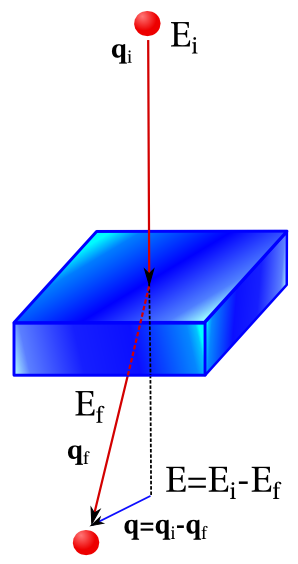
\includegraphics[width=0.2\textwidth]{eels}
  \caption{Dispersion des spectres}\label{fig-dispersion}
\end{wrapfigure}
Comme mentionné dans l'introduction,
la fonction diélectrique du système $\epsilon^{-1}$ est liée aux propriétés optiques et diélectriques d'un matériau.
En fait, dans une vraie expérience de spectroscopie,
on mesure entre autres l'absorption (Abs) et le spectre des pertes en énergie des électrons
(\textit{Electron Energy Loss Spectra}, EELS).
Ces deux grandeurs physiques sont liées à la fonction diélectrique par~\cite{Sottile2003}
\begin{equation}
  \label{eqn-EELS}
  \textnormal{Abs} = \imaginary\qty{\epsilon(\omega, \vb{q})},
  \quad
  \textnormal{EELS} = -\imaginary\qty{\epsilon(\omega, \vb{q})^{-1}}.
\end{equation}
On remarque que la fonction diélectrique est elle-même une fonction de la pulsation de la perturbation externe et du moment de transféré (illustré dans \cref{fig-dispersion}).
Abs nous indique les fréquences de la lumière que le système peut absorber.
EELS nous donne une idée sur les fréquences et les moments
que le système peut échanger avec un projectile venant de l'extérieur (photon ou électron).
Les deux nous donnent donc les caractéristiques intrinsèques du système.
Étant donné que l'inverse de la fonction diélectrique
$\epsilon^{-1}$ est lié à une fonction de réponse linéaire,
la polarisabilité $\chi$, on peut le calculer directement
avec la TDDFT~\cite{Martin2004, Sottile2003}:
\begin{equation}
  \label{epsilon}
  \epsilon^{-1} = 1+ v\chi.
\end{equation}
L'inversion de ce dernier nous donnera la fonction diélectrique $\epsilon$.

La densité du système et la perturbation externe sont liées via $\chi$ par
\begin{equation}
  \delta n(\vb{r}, t) = \int \dd{\vb{r}'} \dd{t'} \chi(\vb{r}, \vb{r}', t-t')\delta V_{\V{ext}}(\vb{r}', t'),
\end{equation}
ou par
\begin{equation}
  \delta n(\vb{r}, \omega) = \int\dd{\vb{r}'}\chi(\vb{r}, \vb{r}', \omega)\delta V_{\V{ext}}(\vb{r}', \omega).
\end{equation}
dans l'espace de Fourier réciproque.
On notera $\chi^0$ et $\chi$ les fonctions de réponse linéaire pour
$V_{\V{tot}}$ et $V_{\V{ext}}$ respectivement (cf. \cref{chap-TRL} pour la définition de ces fonctions).
Les relations entre la fonctionelle de densité $n(\vb{r}, t)$ et les deux potentiels sont

\begin{equation}
  n(\vb{r}, t) = \int \dd{\vb{r}'} \dd{t'} \chi^0(\vb{r}, \vb{r}', t-t') V_{\V{tot}}(\vb{r}', t)
               = \int \dd{\vb{r}'} \dd{t'} \chi(\vb{r}, \vb{r}', t-t') V_{\V{ext}}(\vb{r}', t)
\end{equation}

Enfin, la relation entre $\chi^0$ et $\chi$ peut être donnée de façon plus explicite
en utilisant la méthode variationnelle:
\begin{equation}
  \label{eqn-chi0chi}
  \chi = \frac{\delta n}{\delta V_{\V{ext}}}
       = \frac{\delta n}{\delta V_{\V{tot}}} \frac{\delta V_{\V{tot}}}{\delta n}
       = \chi^0 ( 1 + (v+f_{\V{xc}})\chi)
\end{equation}
où nous avons utilisé l'expression de $V_{\V{tot}}$ dans l'\cref{eqn-Vtot},
$v = \frac{\delta V_H}{\delta n}$ pour la variation du deuxième terme dans l'expression de $V_{\V{tot}}$
(potentiel de Hatree) et $f_{\V{xc}} = \frac{\delta V_{\V{xc}}}{\delta n}$.
À noter que les convolutions sont remplacées par les multiplications ici pour la raison de simplicité d'écriture.

L'intérêt principal de notre travail est donc de prédire le comportement de $\epsilon$ du matériau choisi,
c'est-à-dire de comprendre à quelle énergie et comment le système réagit à une perturbation externe.

Dans la suite de ce rapport, nous allons présenter les aspects numériques de notre projet,
dont les codes qui exploitent les relations décrites dans ce chapitre.
